\subsection{Cập nhật tài liệu và phân tích từ repo đến commit \texttt{58bdfd8}}
\label{sec:repo-update}
Từ commit \texttt{58e28e7} dùng trong lần chạy mẫu đến \texttt{950d47f},
bốn commit bổ sung tài liệu workflow Fiji, kiểm kê Ground Truth và bộ
phân tích công việc 5 của Đức \cite{xlaUpdate950}. Các đầu ra này cung cấp
bối cảnh thực nghiệm và quy trình bàn giao; chúng không thay thế bộ metric
Tầng 2 chuẩn. Hai commit mới nhất sau snapshot trước đã thay đổi giao thức
đánh giá: \texttt{50f65e1} đổi dung sai BSDS từ ô vuông $5\times5$ sang
đĩa Euclidean bán kính 2 pixel (13 pixel), chuyển phép hình thái học trong
bộ đánh giá sang NumPy thuần và giữ ảnh NMS rỗng trong mẫu số với $F_1=0$.
Commit \texttt{58bdfd8} tái tạo số liệu Tier 2 và đồng bộ tài liệu, biểu đồ
và cấu hình theo giao thức mới. Thư mục \texttt{outputs/metrics/duc\_08\_11}
được đánh dấu là snapshot lịch sử trước khi sửa dung sai; nguồn canonical
hiện tại là \texttt{outputs/metrics/PROTOCOL.md} và các CSV cùng thư mục.

\subsubsection{Rà soát trạng thái các nhánh ngày 10/11/2026}
GitHub liệt kê bốn nhánh từ xa. \texttt{dev/NguyenDucManh} đứng tại
\texttt{58bdfd8} và là nguồn canonical hiện hành; \texttt{main} chậm hơn
năm commit và \texttt{fiji/PhamBaoLoc} chậm hơn chín commit. Nhánh
\texttt{thucnghiem/BuiTrungDuc} phân nhánh từ lịch sử cũ, có hai commit
riêng nhưng chậm hơn \texttt{dev} 45 commit; snapshot metric của nhánh này
không thay thế giao thức canonical mới. Nhánh báo cáo
\texttt{report/ieee-gaussian-39e4d02} chỉ có trong checkout cục bộ tại
commit \texttt{a29b82e}; chưa có nhánh cùng tên trên GitHub.

\subsubsection{Phạm vi batch Fiji theo tài liệu mới}
Theo tài liệu workflow đã cập nhật, kho đầu ra Fiji có 435 TIFF float32:
423 bản đồ thuộc phạm vi macro hiện hành và 12 tệp Edge legacy. Nhật ký
có 369 dòng, gồm 303 lệnh một đầu ra và 66 lệnh hai đầu ra; trong số
303 dòng một đầu ra có 12 dòng legacy. Vì vậy phạm vi macro hiện hành
gồm 357 lần gọi và 423 TIFF. Hessian có 14 ảnh, bốn tỷ lệ và hai trị riêng,
tương ứng 56 lần gọi và 112 TIFF. Macro bỏ qua tệp đã có và validator được
chạy riêng sau batch; những con số kiểm kê này không chứng minh mọi TIFF
đã được tạo mới trong cùng một lần chạy.

\subsubsection{Kiểm kê Ground Truth}
Theo tài liệu bàn giao ngày 09/11, mười ảnh BSDS được giữ riêng
5--7 bộ nhãn trên mỗi ảnh, tổng cộng 56 bộ nhãn theo ảnh; con số 56
không đồng nghĩa với 56 người khác nhau. Mỗi ảnh DRIVE có nhãn mạch và
mặt nạ trường quan sát (FOV) riêng. Bốn ảnh blob tổng hợp có bốn đối tượng
mỗi ảnh. Ảnh tế bào \texttt{blob\_05} có 276 đối tượng dương tính đã duyệt
và 15 vùng hình chữ nhật loại trừ; dự đoán có tâm nằm trong vùng loại trừ
được bỏ khỏi ghép nhãn và phép đếm FP theo giao thức tài liệu bàn giao.
Nhãn tế bào do nhóm xây dựng, có gợi ý và kiểm duyệt thủ công; không
xem đây là nhãn chuyên gia chính thức của nhà cung cấp dữ liệu.

\begin{figure*}[tp]
\centering
\begin{minipage}{0.47\textwidth}
\centering
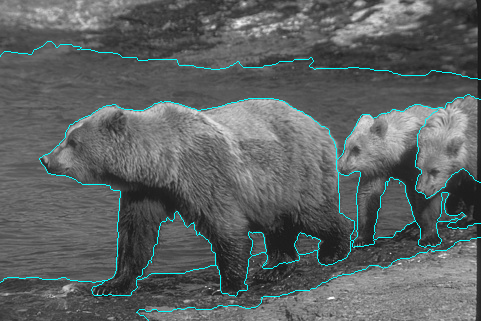
\includegraphics[width=\linewidth]{figures/gt_bsds_01_overlay.png}
\par (a) Biên của một người gán nhãn trên ảnh BSDS.
\end{minipage}
\hfill
\begin{minipage}{0.47\textwidth}
\centering
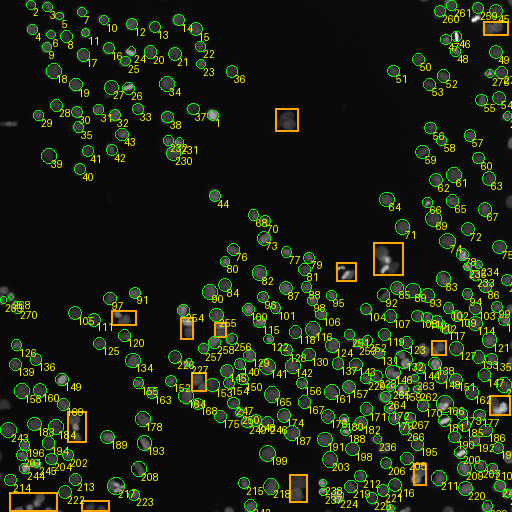
\includegraphics[width=\linewidth]{figures/gt_blob_05_overlay.png}
\par (b) Tâm, bán kính và vùng loại trừ trên ảnh tế bào.
\end{minipage}
\caption{Minh họa Ground Truth do nhóm cung cấp trong
\texttt{docs/09\_11/ground\_truth\_figures}: đường cyan ở (a) là nhãn
của annotator 01 trong sáu bộ nhãn của ảnh; vòng xanh và khung cam ở (b)
biểu diễn đối tượng và vùng loại trừ. Overlay dùng để minh họa,
không được thay thế mask hoặc JSON gốc khi tính chỉ số.}
\label{fig:gt-handoff}
\end{figure*}

\subsubsection{Số liệu Tầng 2 theo giao thức canonical hiện tại}
Commit \texttt{58bdfd8} tái tạo metric trong \texttt{outputs/metrics/}
theo dung sai đĩa Euclidean. Các F1 BSDS dưới đây và cặp ngưỡng lấy từ
\texttt{PROTOCOL.md}; bảng Python--Fiji DRIVE/Blob và số đếm micro lấy từ
\texttt{tier2\_results\_both.csv}. Kết quả Python Blob chính thức ở lưới
8 mức được lưu riêng trong \texttt{tier2\_results.csv}.

\begin{table*}[htbp]
\centering
\caption{F1 theo bộ metric canonical tại commit \texttt{58bdfd8}.}
\label{tab:repo-canonical-f1}
\begin{tabular}{lrrr}
\toprule
Tác vụ / tỷ lệ & Python & Fiji & $\Delta F_1$\\
\midrule
BSDS $\sigma=1$ & 0.455418 & 0.455478 & $+0.000060$\\
BSDS $\sigma=2$ & 0.477886 & 0.477886 & $0.000000$\\
BSDS $\sigma=4$ & 0.441491 & 0.441491 & $0.000000$\\
BSDS $\sigma=8$ & 0.343340 & 0.343340 & $0.000000$\\
DRIVE, macro & 0.680633 & 0.681651 & $+0.001019$\\
DRIVE, micro & 0.682895 & 0.683897 & ---\\
Blob, macro & 0.893023 & 0.891901 & $-0.001122$\\
Blob, micro & 0.492114 & 0.486656 & ---\\
\bottomrule
\end{tabular}
\end{table*}

Với BSDS $\sigma=\{1,2,4,8\}$, cặp $(p_{low},p_{high})$ lần lượt là
$(76,94)$, $(67,91)$, $(49,80)$ và $(23,50)$; F1 tham chiếu FeatureJ Edges
lần lượt là $0.488766$, $0.500818$, $0.464873$ và $0.354292$. Ngưỡng được
chọn trên Python rồi giữ nguyên cho Fiji, nên đây không phải điểm kiểm tra
độc lập. DRIVE được chấm trong FOV đã xói mòn $\lceil4\sigma\rceil$.
Blob dùng ghép một-một, tâm trong 2 pixel, bán kính sai không quá 20%, và
bỏ dự đoán có tâm trong vùng ignore. Bảng macro Python--Fiji dùng cấu hình
chung 7 mức. Riêng kết quả Python chính thức cho \texttt{blob\_05} ở lưới
8 mức là 140/329 ghép đúng/dự đoán ($F_1=0.4628$); Fiji fair 7 mức là
139/329 ($F_1=0.4595$). Hàng Python 7 mức 140/326 ($F_1=0.4651$) vẫn có
trong CSV so sánh lưới chung, nhưng không phải kết quả Python chính thức
dùng làm headline. Các micro F1 được tính từ tổng số đếm trong CSV.

\subsubsection{Hiệu quả chập tách rời}
Benchmark đo chập 2D trực tiếp so với hai chập 1D tách rời cho Gaussian,
$L_x$ và $L_{xx}$, trên ba ảnh mẫu và bốn tỷ lệ, tổng cộng 36 trường hợp với
5 lần lặp mỗi trường hợp. Theo CSV
\texttt{outputs/metrics/optimization\_benchmark.csv}, tốc độ nhanh hơn
nằm trong khoảng $1.375738$ đến $31.392971$ lần tùy ảnh, tỷ lệ và toán tử;
sai khác tuyệt đối lớn nhất là $1.279\times10^{-12}$
\cite{xlaOptimizationBenchmark}. Mức tăng tốc quan sát
không cần bằng đúng tỷ số số phép toán lý thuyết: phép đo còn chịu ảnh hưởng
của kích thước kernel, overhead Python và quản lý bộ nhớ. Đây là benchmark
trên ba ảnh mẫu, không phải cam kết tốc độ trên toàn bộ dữ liệu hay máy khác.

\subsubsection{Cấu hình FeatureJ Derivatives}
Tài liệu Fiji mới ghi tham số hệ số cắt kernel $k=3$ cho Gaussian và
$k=4$ cho đạo hàm bậc 1--2, biên phản chiếu \texttt{mirror}, và đầu ra
FeatureJ là giá trị thô, không nhân thêm $\sigma^n$. Vì đây là quy ước
riêng được ghi trong workflow hiện tại, cần nêu rõ khi tái lập hoặc so với
nhánh NumPy có chuẩn hóa tỷ lệ; không được coi ảnh chụp GUI là phép xác nhận
độc lập cho toàn bộ benchmark.

\subsubsection{Tiêu chí nghiệm thu Tầng 1}
Trong metric snapshot mới, 35/220 cặp đạt đồng thời ngưỡng gốc
$\mathrm{rel\_err}<10^{-4}$ và Pearson $>0.9999$; 185 cặp còn lại
\emph{chưa đạt ngưỡng gốc}. Các nhãn \texttt{RELAXED} trong snapshot trước
chỉ mô tả kết quả theo ngưỡng nới lỏng của báo cáo, không phải xác nhận
nhóm đã chấp nhận thay đổi tiêu chí nghiệm thu. Tương quan cao không đủ
để kết luận sai số biên độ thỏa chuẩn.

